% Fork from Gemini theme
% See: https://github.com/alfurka/gemini-uq
% 	   https://github.com/anishathalye/gemini


\documentclass[final]{beamer}
% ACoP req: 36 inches (91.5 cm) wide x 48 inches (122 cm) high 
% ====================
% Packages
% ====================

\usepackage{fontspec}
\usepackage{lmodern}
\usepackage[size=custom,width=91.5,height=122,scale=1.0]{beamerposter}
\usetheme{uofmn}
\usecolortheme{uofmn}
\usepackage{graphicx}
\usepackage{booktabs}
\usepackage{tikz}
\usepackage{pgfplots}
\pgfplotsset{compat=1.17}

% ====================
% Lengths
% ====================

% If you have N columns, choose \sepwidth and \colwidth such that
% (N+1)*\sepwidth + N*\colwidth = \paperwidth
\newlength{\sepwidth}
\newlength{\colwidth}
\newlength{\verwidth} 
\setlength{\verwidth}{0.04\paperwidth} 
\setlength{\sepwidth}{0.03\paperwidth}
\setlength{\colwidth}{0.3\paperwidth}

\newcommand{\separatorcolumn}{\begin{column}{\sepwidth}\end{column}}

% ====================
% Title
% ====================

\title{Evaluation of Recorded Time Deviations on Parameter Estimates\\ in Nonlinear Mixed-effect Analyses}

\author{\emph{Mutaz M.} \textbf{Jaber} \inst{1} \and \emph{Mahmoud} \textbf{Al-Kofahi} \inst{1} \and \emph{Richard C.} \textbf{Brundage}\inst{1}}

\institute[shortinst]{\inst{1} Department of Experimental and Clinical Pharmacology, College of Pharmacy, University of Minnesota 
%\samelineand \inst{2} Metrum Research Group
%\samelineand \inst{3} Gilead Sciences
}

% ====================
% Footer (optional)
% ====================

\footercontent{
  \href{https://www.example.com}{https://www.umn.edu/\~jaber038} \hfill
  ACoP13 Conference 2022, Colorado --- STPM506 \hfill
  \href{mailto:a.kalay@example.com}{Mutaz Jaber, jaber038@umn.edu}}
% (can be left out to remove footer)

% ====================
% Logo (optional)
% ====================

% use this to include logos on the left and/or right side of the header:
% \logoright{\includegraphics[height=7cm]{logo1.pdf}}
% \logoleft{\includegraphics[height=7cm]{logo2.pdf}}

% ====================
% Body
% ====================

\begin{document}
\addtobeamertemplate{headline}{}
{
    \begin{tikzpicture}[remember picture,overlay]
      \node [anchor=north west, inner sep=3cm] at ([xshift=0.0cm,yshift=0.5cm]current page.north west)
      {
\includegraphics[height=6.0cm]{logos/Logo-Left.png}}; % also try shield-white.eps
      \node [anchor=north east, inner sep=3cm] at ([xshift=0.0cm,yshift=0.5cm]current page.north east)
      {
\includegraphics[height=4.0cm]{logos/Logo-Right.png}};
    \end{tikzpicture}
}

\begin{frame}[t]
\begin{columns}[t]
\separatorcolumn

\begin{column}{\colwidth}

  \begin{alertblock}{\textbf{SUMMARY}}

An assumption that clinical data are recorded without any error is optimistically made. While some study personnel will record the actual times when there is a deviation others record the nominal time. In the current modeling and simulation work we:
\begin{itemize}
\item[I] Investigate an approach that includes error correction factor on recorded time and quantitate the bias in estimated parameters.
\item[II] Determine the maximal deviation between observed and recorded times that does not cause significant bias. 
\item[III] Compare the performance of first-order conditional (FOCE) and stochastic expectation-maximization (SAEM) algorithms in handling data with erroneous recorded times. 
\end{itemize} 
We conclude that:
\begin{itemize}
    \item Adding a correction factor to the nominal time will lead to diluting the bias and imprecision in PK estimates compared to assuming the nominal time is absolute.
    \item A magnitude difference greater than 5 minutes between the actual and nominal times can lead to more than 10\% bias and imprecision PK estimates.
    \item In comparison between estimation algorithms, SAEM estimates were more accurate than FOCE in primary PK parameters and produced similar RUV estimates on average. 
\end{itemize}

Despite the limited settings, we believe this work provides general insight on the ways to handle suspected data with unrecorded time deviations.

  \end{alertblock}
  \begin{block}{\textbf{METHODS}}
Two sources of error were modeled in this work: a classical error model and a combined classical and Berkson error model. The former is what the pharmacometrician/clinical pharmacologist frequently implements in NLMEM to characterize the errors in observed concentrations. The general structure for the $j^{th}$ subject and $i^{th}$ time point as:
\begin{equation}\label{eq:1}
y_{i,j} = f(\Phi, x_i, t_{i,j}) + g(\Phi, x_i, t_{i,j}, \zeta)\epsilon_{i,j}
\end{equation}  
Let us introduce the actual time $T_A$ for the $i^{th}$ concentration in the $j^{th}$ subject as a function of nominal time   $T_N$ and gaussian noise, $\kappa$, that is an independent and identically distributed random variable with mean 0 and standard deviation $K$, representing the deviation of actual time from the nominal time.
\begin{equation}\label{eq:two}
	T_{A,i,j} = T_{N,i,j} + \kappa_{i,j} 
\end{equation}
Therefore, the kappa model, $M_\kappa$, can be presented as:
\begin{equation}\label{eq:three}
y_{i,j} = f(\Phi, x_i, T_{A,i,j}) + g(\Phi, x_i, T_{A,i,j}, \zeta)\epsilon_{i,j}
\end{equation}  
In order to evaluate if there is a threshold of time deviation that is acceptable, we will be defining $t^*$ in this work to represent the time used in estimation process under parts II-III, where this a mathematical case:
\begin{equation}\label{eq:for}
t^* = \begin{cases} T_A & |T_A - T_N| > \delta \\ T_N & \mathrm{otherwise} \end{cases}
\end{equation} 

A 500 mg single dose study with 500 in-silico subjects were simulated under a two-compartment first-order absorption and linear elimination model, $f(.)$. Individual pharmacokinetic parameters were sampled from a multivariate log-normal distribution with a mean of the logarithmic typical values vector and diagonal variance matrix $\Omega$. A 15\% CV served as a baseline residual unexplained variability (RUV) using a proportional error model $g(.)$. Table \ref{tab:1} presents the true simulated PK parameters with corresponding BSV CV, and RUV magnitude.   
\begin{table}
		\label{tab:1}
      \centering
      \begin{tabular}{l r r c}
        \toprule
        \textbf{Parameter} & \textbf{Estimate} & \textbf{BSV} \\
        \midrule
        CL (L/hr) & 3.5 & 30\% \\
        V (L)& 20.0 & 30\% \\
        Q (L/hr)& 5.0 & 30\%  \\
        Vp (L)& 50.0 & 30\% \\
        Ka (1/hr)& 0.7 & 30\% \\
        \bottomrule
      \end{tabular}
      \caption{Pharmacokinetic parameter values with corresponding between-subject variability reported as coefficient of variation. }
    \end{table}
Three sample collection designs were examined; (a) Intense design (I) with 8 samples: 0.5, 1, 2, 4, 8, 12, 24, 48 hours post dose, (b) sparse design (S) with 4 samples: 0.5, 2, 24, 48 hours post dose and (c) mixed design (M) with 33\% of subjects having 8 samples as in I, 33\%  of subjects having 6 samples (0.5, 2, 4, 12, 24, 48), and 33\% of subjects having 4 samples as in S.\par
Two models were created: the null model (Eq \ref{eq:1}; $M_0$), and the kappa model, (Eq \ref{eq:three};  $M_\kappa$), respectively. Model was built with `PRED` subroutine to allow the implementation of $M_\kappa$ since PRED has the flexibility of writing the analytical solution for the two-compartment model. Parameters were estimated using first-order conditional estimation (FOCE) with interaction between $\eta$ and $\epsilon$ since a proportional error model is used.\par
In part two, simulations were perturbed with standard deviation of 10 minutes  in time, then followed by creating a new column in the dataset presenting the time used in the estimation process as shown in equation (Eq \ref{eq:for}; $t^*$). The difference, $\delta$, was selected to be 5, 10, 15, or 30 minutes. In fitting the model to the data, $t^*$ was used as the independent variable time with $M_0$.\par
In part 3 of this study we re-used data generated from the previous section (part II) but with different estimation methods; either with FOCE or SAEM algorithms including interaction. The AUTO=1 criteria was used to select the most suitable convergence test in SAEM, and importance sampling was used to evaluate the likelihood function.
  
  \end{block} 

\end{column}
\separatorcolumn

\begin{column}{0.6\paperwidth}
\begin{block}{\textbf{RESULTS}}
%~\vskip2cm
\begin{figure}
\centering
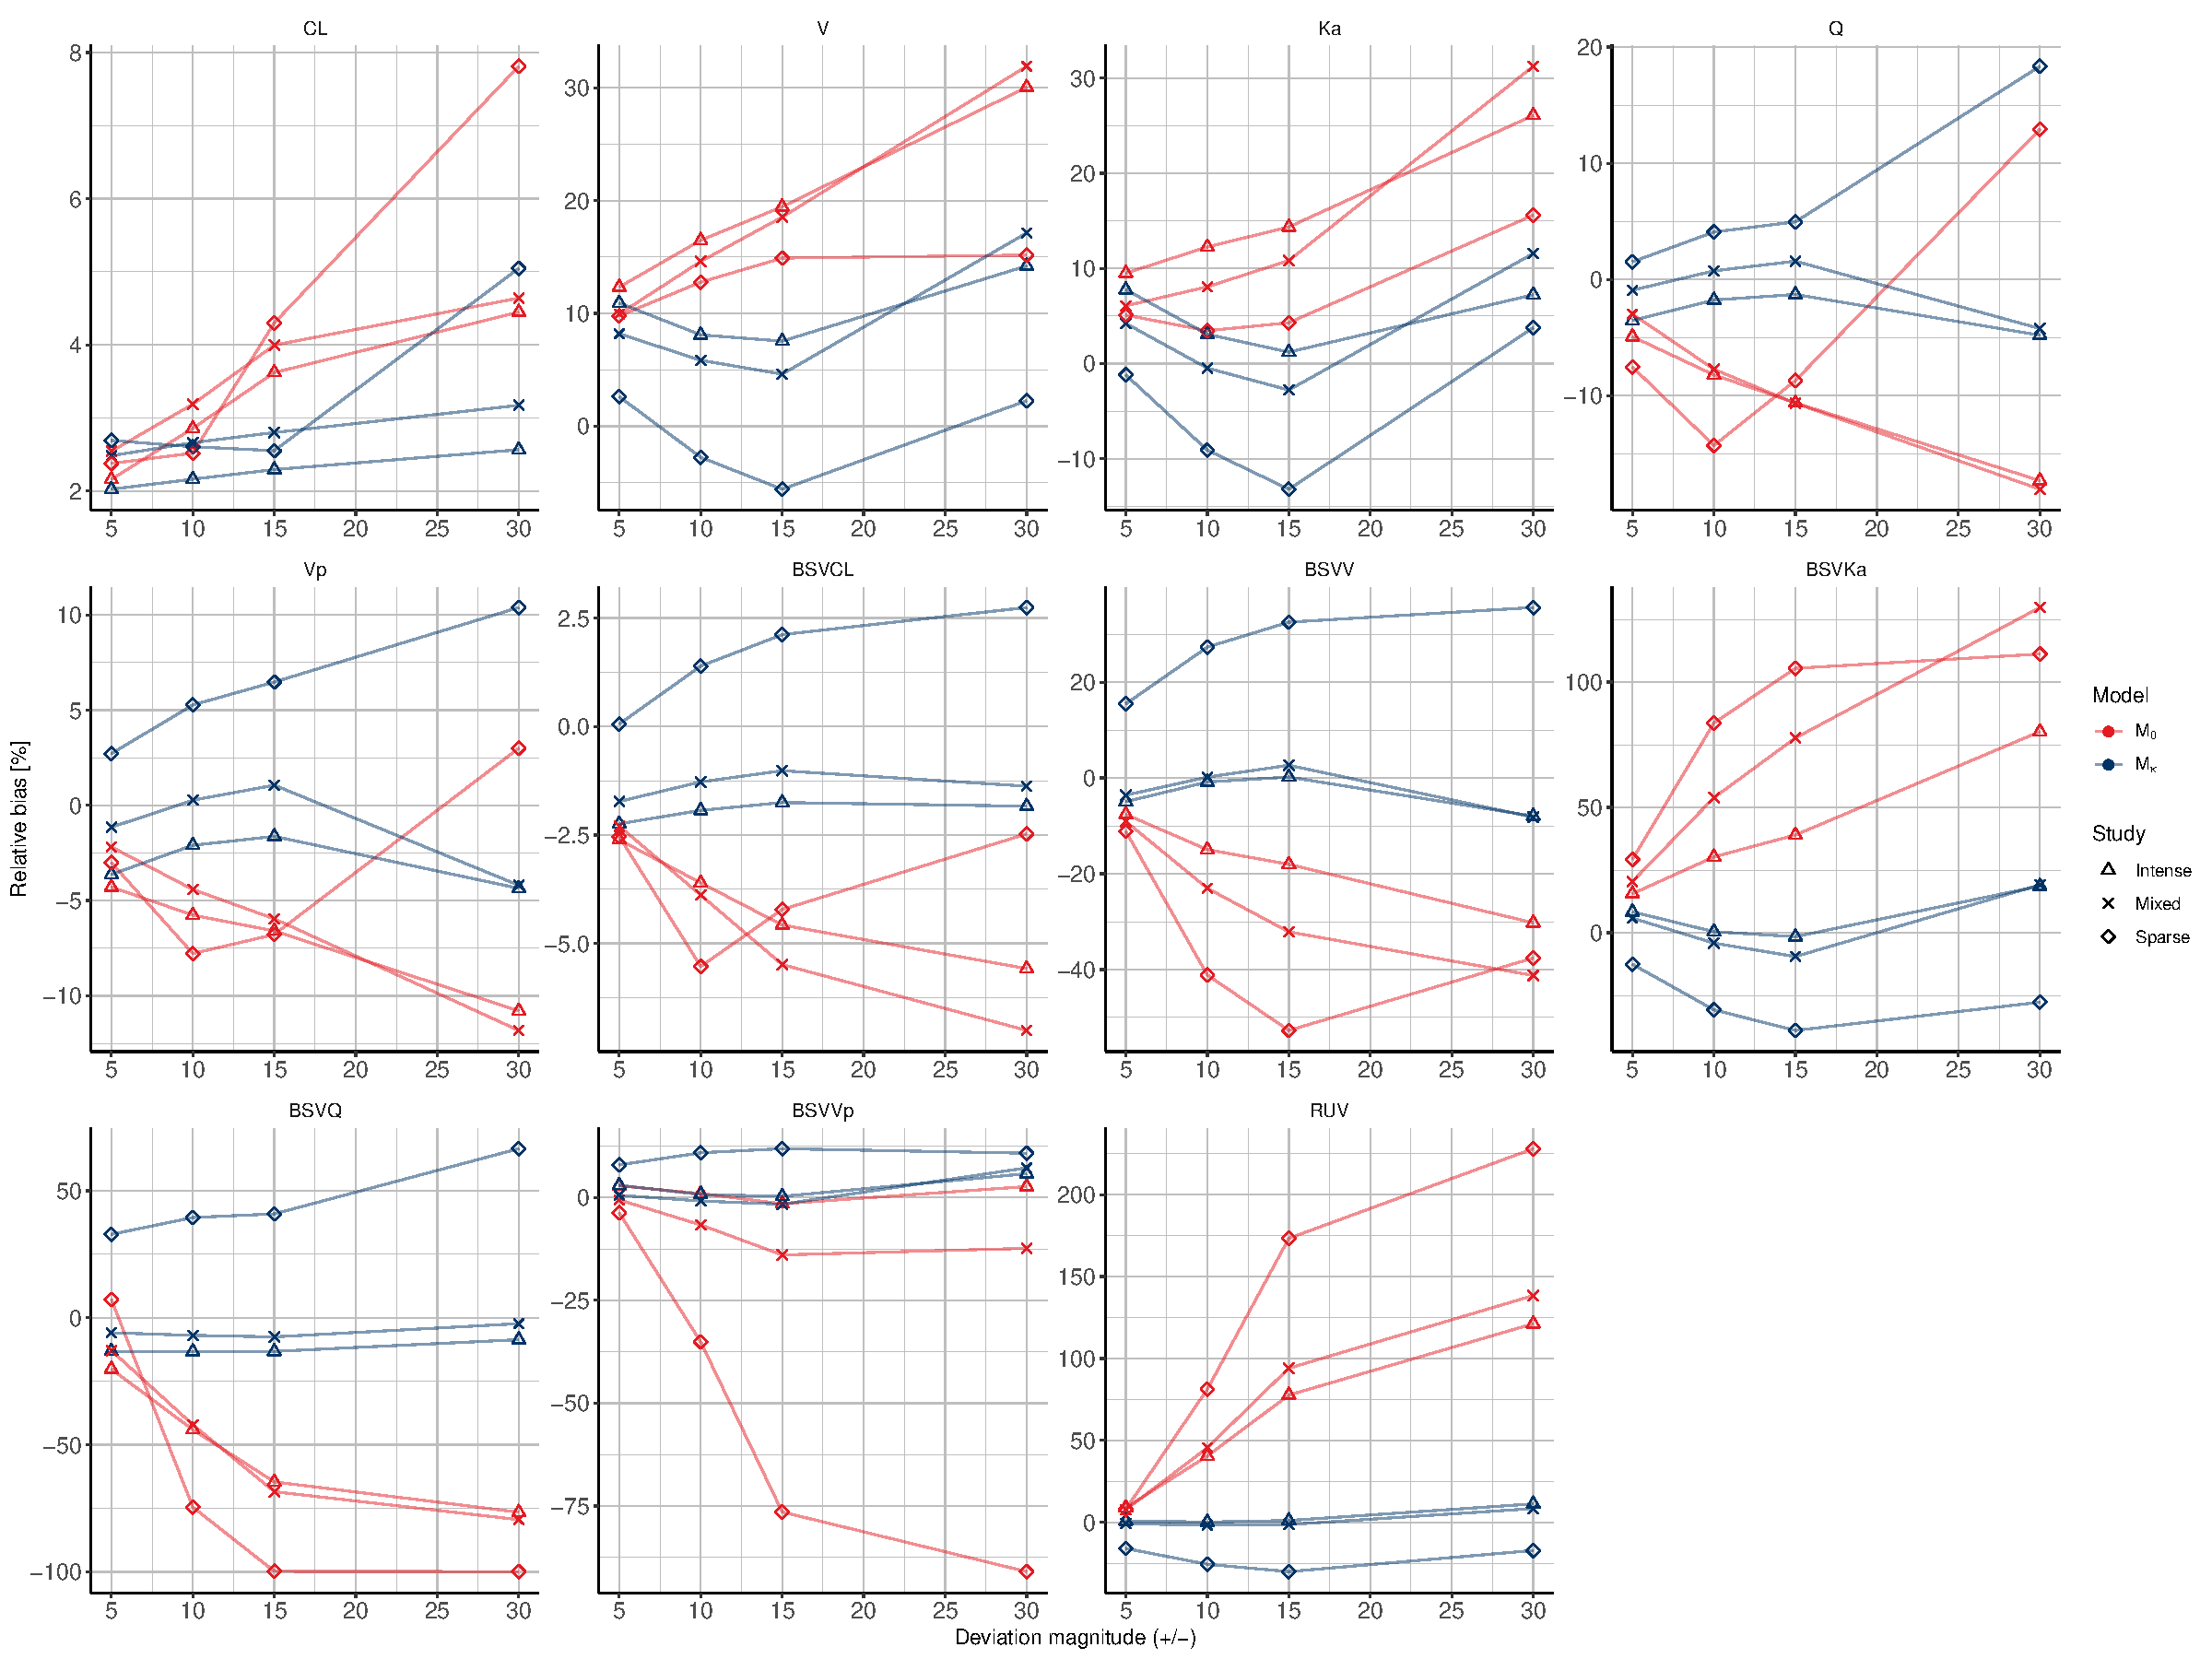
\includegraphics[width=55cm]{Figure1A}
\caption{Comparison of the relative bias for the null model $M_0$ and kappa model $M_K$ stratified on study design}
\end{figure} 
\begin{figure}
\centering
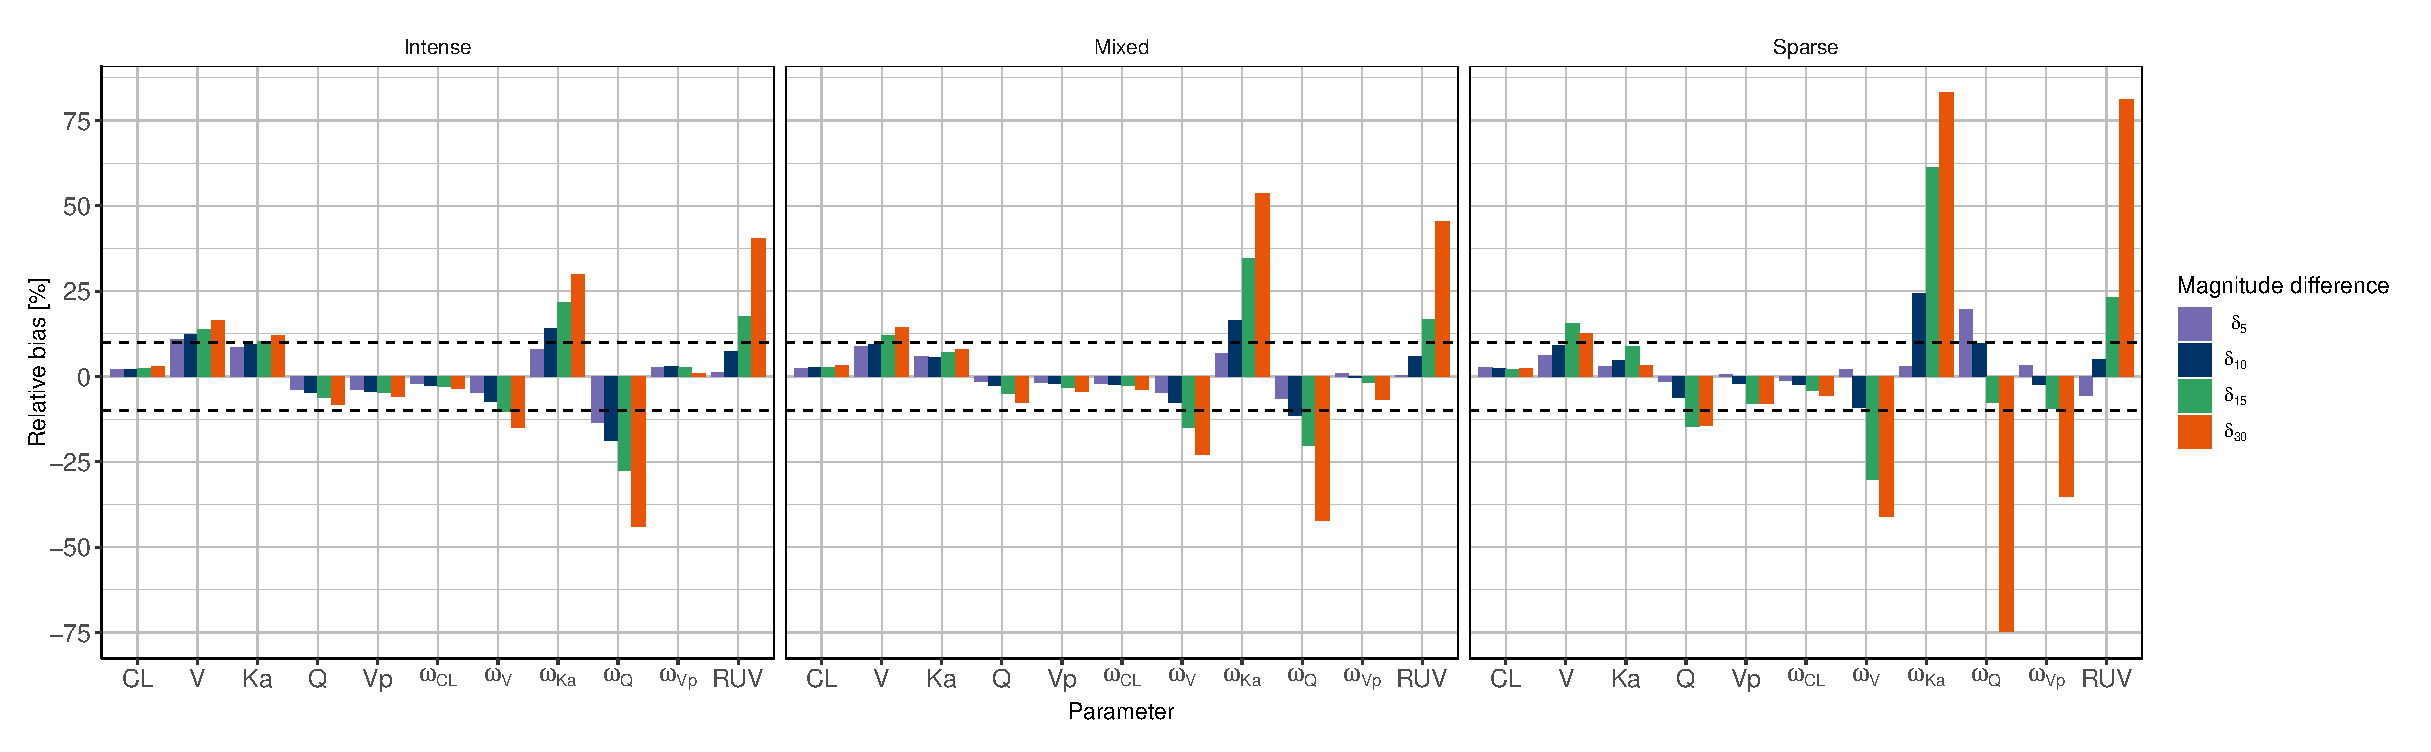
\includegraphics[width=55cm]{Figure3A.eps}
\caption{The magnitude difference $\delta$ between the true time and recorded time. }
\end{figure} 
\begin{figure}
\centering
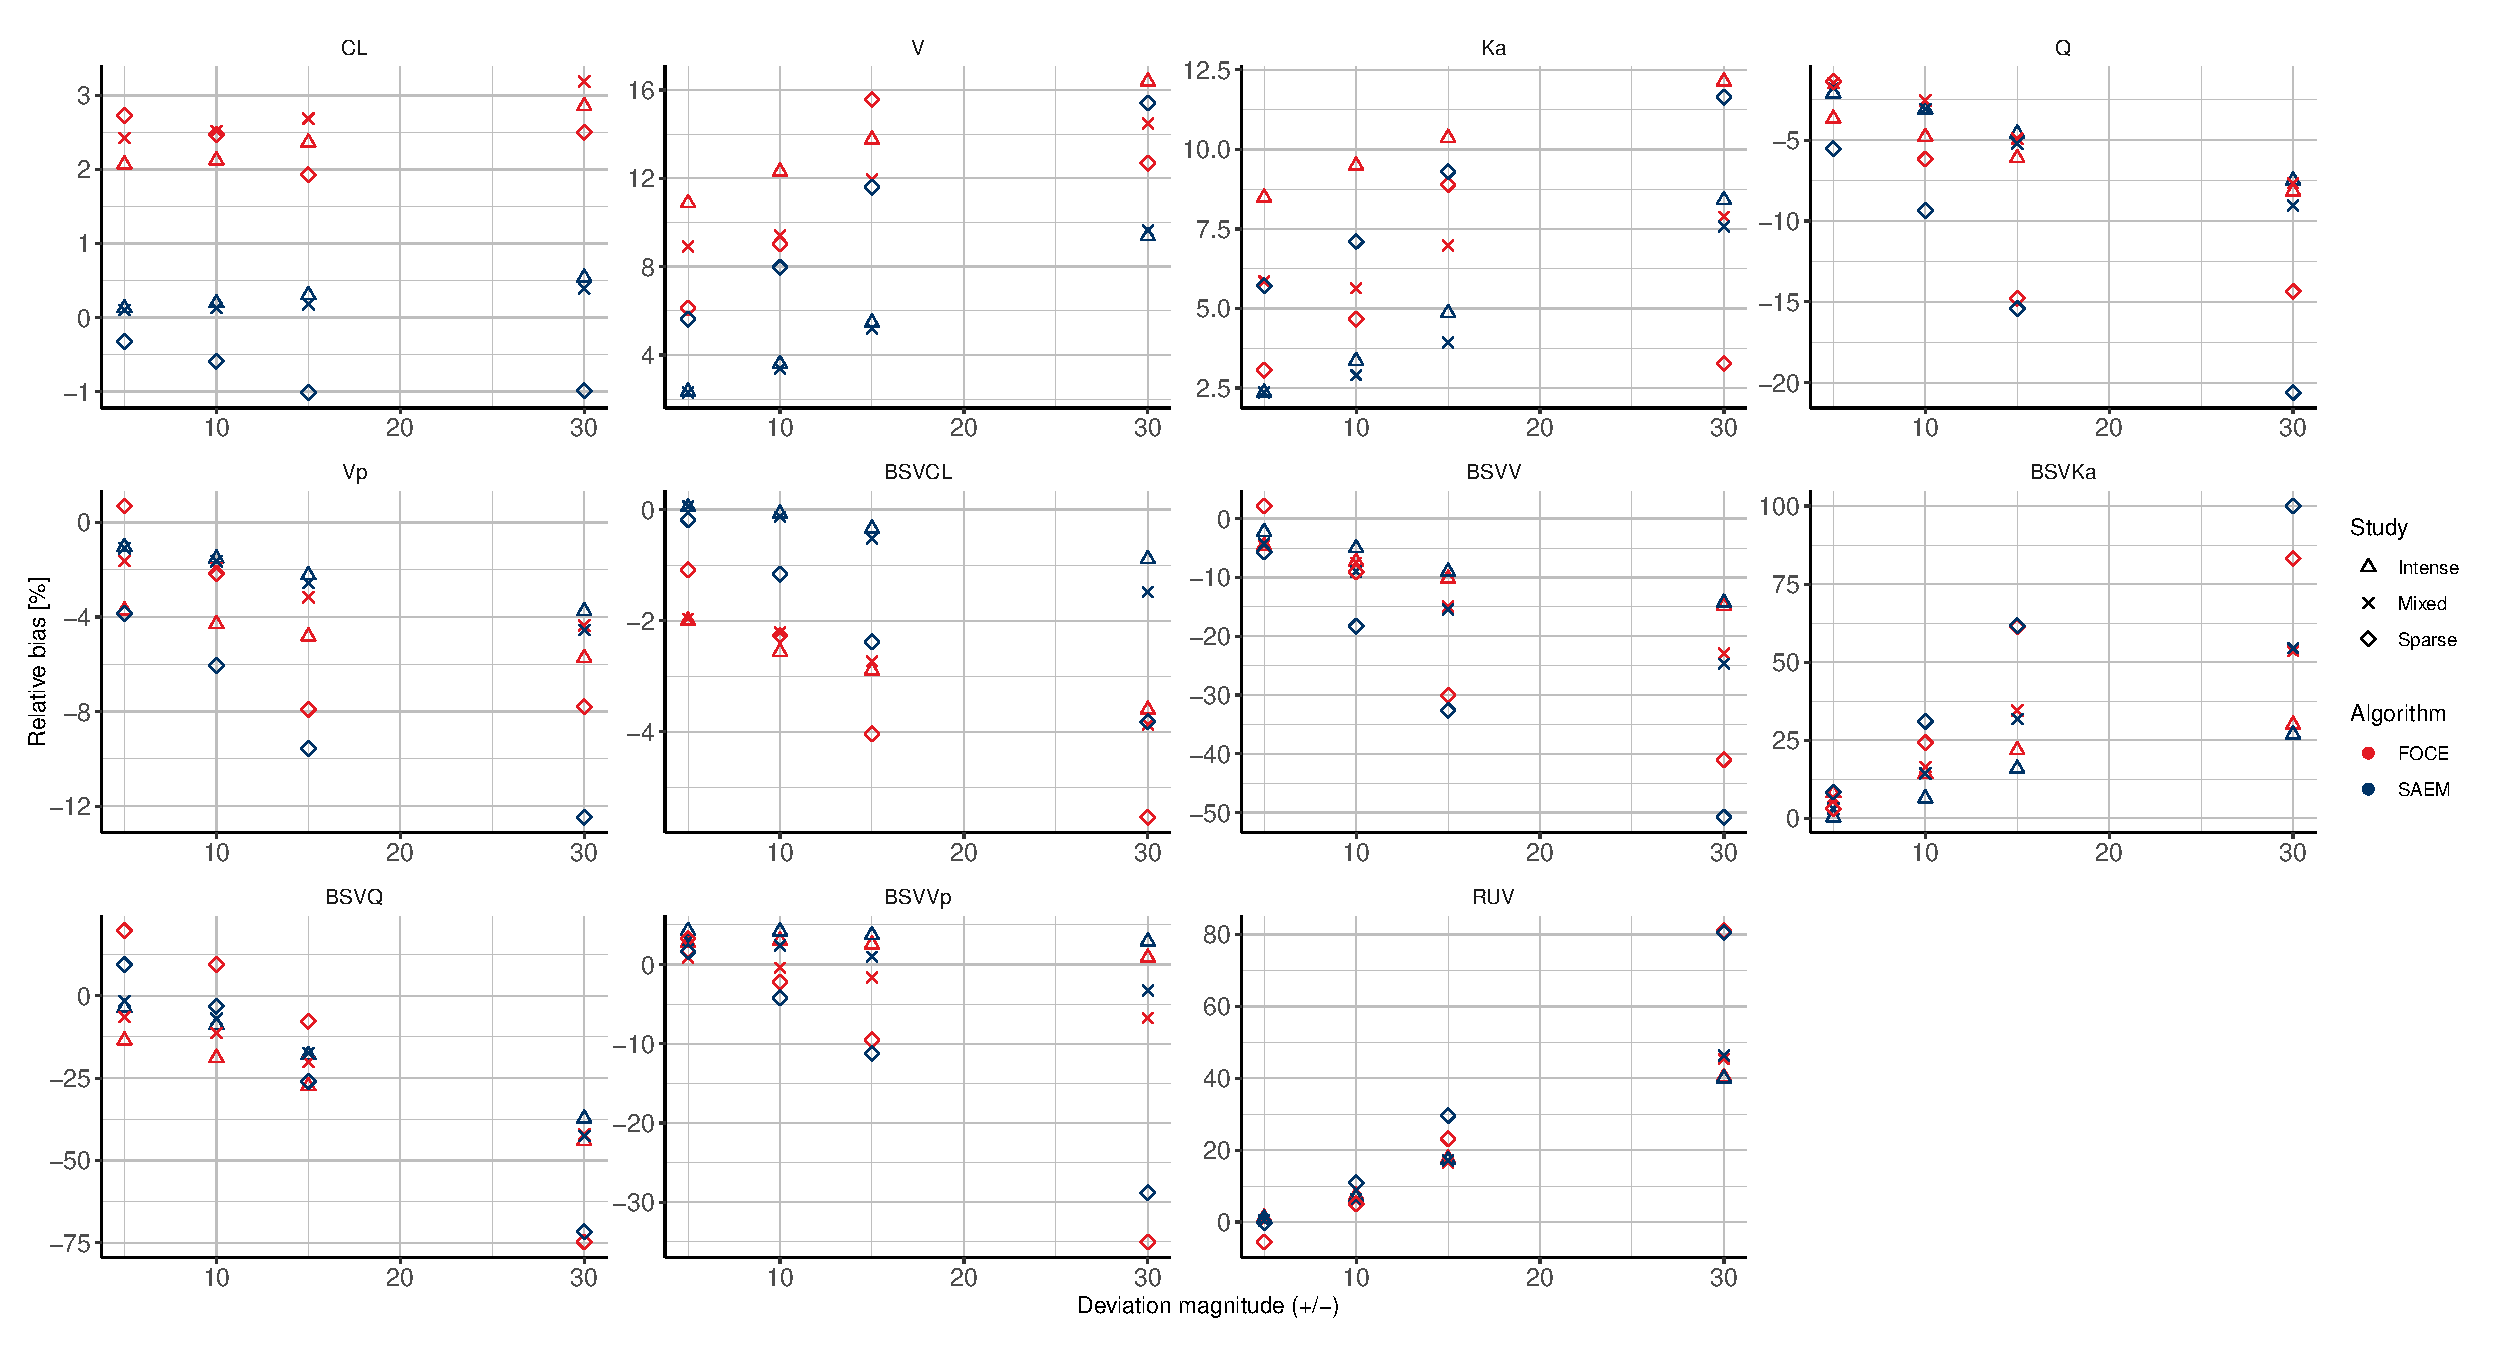
\includegraphics[width=55cm]{Figure4.eps}
\caption{Comparison between FOCE and SAEM in handling erroneous times stratified on sample collection design. First-order conditional estimation (red) and stochastic approximation expectation-maximization (blue).}
\end{figure} 
\end{block}

\end{column}

\end{columns}
\end{frame}

\end{document}
